\documentclass[11pt]{article}
\usepackage{amsmath}
\usepackage[margin=0.68in]{geometry}
\usepackage{booktabs}
\usepackage{enumitem}
\usepackage{fancyhdr}
\usepackage{graphicx}
\usepackage[table]{xcolor}
\usepackage[hidelinks]{hyperref}
\usepackage{listings}
\usepackage{microtype}
\usepackage{tabularx}
\usepackage{titlesec}
\graphicspath{{docs/design/drafts/lesson-039/}{./}}
\definecolor{Ink}{gray}{0}
\definecolor{CodeGray}{gray}{0.96}
\hypersetup{hidelinks,pdftitle={ADK Lesson 039: Percussion Sequencer},
 pdfauthor={Kevin Shanahan},
 pdfsubject={Deterministic grouping, acoustic association, quantization, and playback intents},
 pdflang={en-US}}
\pagestyle{fancy}\fancyhf{}
\lhead{\textsc{ADK Lesson 039}}\rhead{Percussion Sequencer}
\cfoot{\thepage}\setlength{\headheight}{14pt}
\setlength{\parindent}{0pt}\setlength{\parskip}{5pt}
\setlist{nosep,leftmargin=1.45em}
\titleformat{\section}{\Large\bfseries\color{Ink}}{\thesection}{0.5em}{}
\lstdefinestyle{adkcpp}{language=C++,backgroundcolor=\color{CodeGray},
 basicstyle=\ttfamily\small,keywordstyle=\color{Ink}\bfseries,
 commentstyle=\color{Ink},columns=fullflexible,keepspaces=true,
 showstringspaces=false,frame=single,rulecolor=\color{Ink},
 breaklines=true,tabsize=4}
\newcommand{\lessonbox}[1]{%
 \begin{center}\fcolorbox{Ink}{white}{\parbox{0.92\linewidth}{#1}}\end{center}}

\begin{document}
\lessonbox{\textbf{NONCANONICAL DESIGN DRAFT --- NOT PUBLISHED.} This file is
review material under \texttt{docs/design/drafts}. It is not a released
lesson, site page, download, Mega example, schematic, physical acceptance
record, or support claim. Promotion requires relocation into canonical paths
and every applicable acceptance gate.}

\begin{center}
 {\Huge\bfseries Percussion Sequencer}\\[4pt]
 {\Large Group supplied attacks, associate one envelope, replay bounded cues}\\[8pt]
 \textit{Logical lanes and deterministic time; no physical specimen required}
\end{center}
\begin{tabularx}{\linewidth}{@{}>{\bfseries}l X >{\bfseries}l X@{}}
Lesson & 039 --- project & Time & 180--240 minutes\\
Prerequisites & Lessons 037 and 038 & Board & host fixture\\
Evidence & snapshots, operation traces, LED/step/tone intents &
Status & host-independent draft; physical acceptance open\\
Energy class & E0 project engine and supplied four-lane traces\\
\end{tabularx}

\lessonbox{\textbf{Scope gate.} This lesson operates on one narrow project
evidence record: a four-bit attack mask, one status for each surface, one
acoustic-source status, and an optional copied acoustic completion. Logical
surface numbers are not physical instruments. LED, step-display, heartbeat,
and tone values are presentation intents only. ``Silent'' means the model
publishes zero tone frequency and duration; it does not prove a piezo, speaker,
board, or room is physically silent.}

\section{Mission and vocabulary}
The project composes the two earlier behaviors:
\[
\text{qualified contacts}\rightarrow\text{bounded group}\rightarrow
\text{one acoustic association}\rightarrow\text{quantized hits}
\rightarrow\text{playback frame}.
\]
It teaches correlation without claiming force, acceleration, calibrated
sound pressure, speech content, specimen identity, or a performed rhythm.
The engine owns no pins, timers, endpoints, clock, callback, dynamic storage,
or persistence. Every update receives a complete value record and supplied
time.

\section{Build one group from four logical lanes}
\begin{center}
% ADK visual: pencil
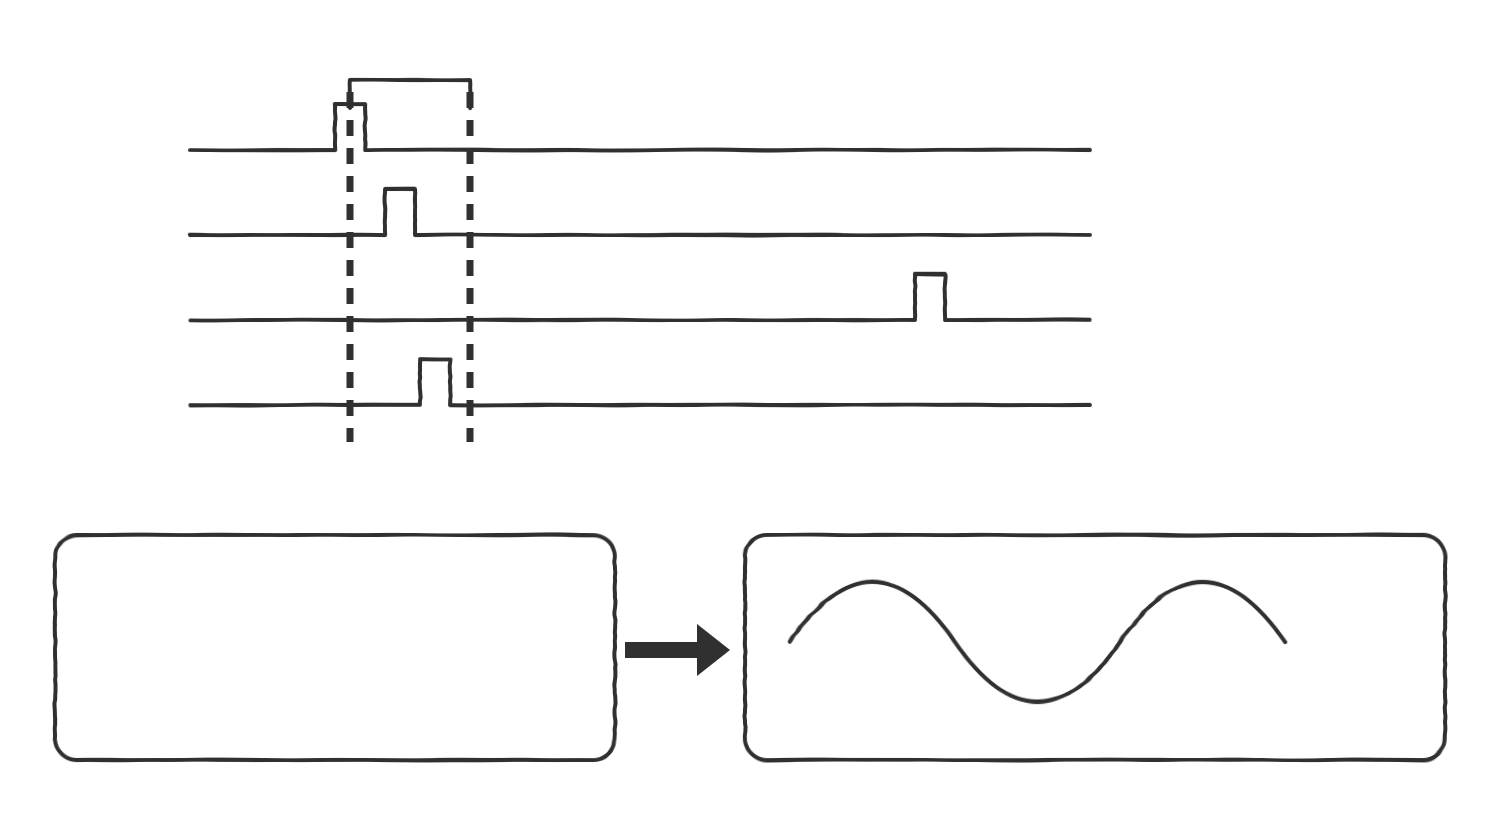
\includegraphics[width=0.98\linewidth]{039-logical-lanes-pencil.png}

\small Top to bottom: logical surfaces 0, 1, 2, and 3. The bracket and two
dashed vertical bounds mark the inclusive group. The lower left box is the pending group;
the heavy right arrow leads to the lower right completed-envelope association.

\small\textit{Alternative text: four supplied logical contact traces enter an
inclusive simultaneous window. Surfaces zero, one, and three form one pending
group in ascending surface order. A later surface-two attack is suppressed
while the closed group waits. One eligible completed acoustic window supplies
relative intensity to the whole group; timeout instead finalizes zero
intensity.}
\end{center}

Recording begins with the first consumable contact attack. That attack freezes
the recording tempo and epoch. At most one attack from each of four surfaces
enters the pending group. An attack exactly at the simultaneous-window
boundary belongs to that group. The group closes on the first later update at
or beyond the boundary.

Only one closed group may wait for association. A new attack during that wait
sets \texttt{hitSuppressed}; it is not secretly queued. The first eligible
completed acoustic interval whose inclusive start-to-end range contains the
first attack supplies one relative intensity to every group member. At the
association-timeout boundary, timeout wins and finalizes intensity zero.
Each completion may satisfy only the oldest pending group and only on its
completion update.

\begin{tabularx}{\linewidth}{@{}l X@{}}
\toprule
Project evidence field & Consumable meaning\\
\midrule
\texttt{attackMask} & bits 0--3 are copied qualified attacks; upper bits are invalid\\
\texttt{surfaceStatus[4]} & exact upstream outcome for each logical lane\\
\texttt{acousticStatus} & exact upstream acoustic-source outcome\\
\texttt{acousticCompletion.present} & whether one copied completion is supplied\\
\texttt{eventStartedAt/eventDuration/intensity} &
bounded completion interval and relative intensity when present\\
\bottomrule
\end{tabularx}

The project does not reinterpret component phase or quality enums. It trusts
the adapter to publish only qualified attack bits and an eligible completed
interval, while preserving exact upstream statuses. The first non-Ok surface
in lane order is attributed as \texttt{Surface0} through \texttt{Surface3};
an acoustic failure is attributed as \texttt{Acoustic}. Invalid masks and
noncanonical absent-completion fields are attributed as project
\texttt{Input} or \texttt{Acoustic} evidence. Timing and tempo have their own
\texttt{PercussionFaultSource} values. A fault clears frame and tone intents
immediately and retains finalized hits for diagnosis.

\section{Quantize the pattern}
The recording grid contains 4--16 sixteenth-note steps. Tempo is bounded
between 30 and 240 beats per minute. With integer milliseconds:
\[
\mathrm{stepPeriod}=\left\lfloor
\frac{60000}{\mathrm{tempoBpm}\times4}\right\rfloor .
\]
The remainder is deliberately truncated. Each attack is quantized to the
nearest step relative to the recording epoch; an exact half-step tie rounds
forward. Members of one group share its first attack time and are stored in
ascending surface order.

Different surfaces may share a step. A repeated attack from one surface at
that same quantized step is suppressed. Final hits are ordered by step,
surface, then bounded ordinal. The fixed pattern holds 32 hits. Capacity is
atomic after duplicate removal: when every new member cannot fit, the entire
group is suppressed. No member is inserted, no ordinal advances, and existing
hits never move or change.

Finalized hits are not exposed as an internal array. \texttt{hit(index)}
returns a copied \texttt{Result<PercussionHit>} for
\(0\leq\texttt{index}<\texttt{hitCount}\) and
\texttt{InvalidArgument} otherwise. Every returned hit includes
\texttt{AcousticCompletion} or \texttt{AssociationTimeout} provenance.
\texttt{lastAssociation} is transient finalization evidence, not durable
per-hit provenance.

\section{Play the frame current now}
\begin{center}
% ADK visual: pencil
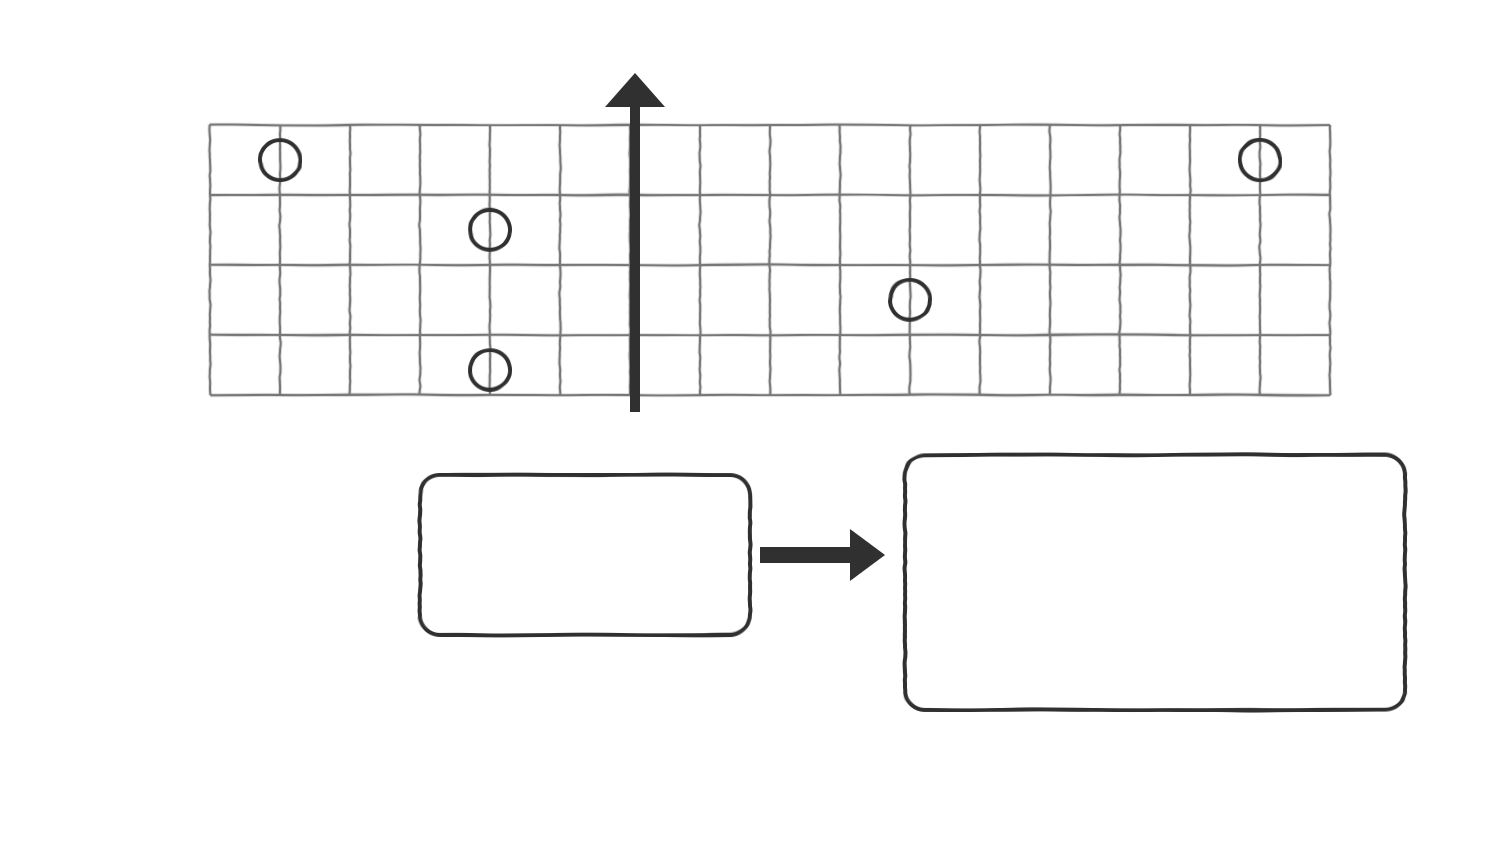
\includegraphics[width=0.74\linewidth]{039-quantized-playback-pencil.png}

\small Grid rows are logical surfaces 0--3; columns are steps 0--15. The heavy
vertical bar with triangular pointer is the current-step cursor. The lower
left box is the current frame; its heavy right arrow leads to the lower right
LED, step-display, heartbeat, and bounded-tone intents.

\small\textit{Alternative text: a sixteen-step pencil grid contains five
logical hits across four lanes, including two lanes sharing step four. A
current-step cursor selects one frame. The frame drives surface-LED, step,
heartbeat, and bounded-tone intents. A note explains that sparse updates jump
to the current frame and never replay missed cues late.}
\end{center}

\texttt{playEvent} toggles recording and playback. Empty playback is an
idempotent no-op. Each playback start creates a new playback epoch and
publishes step zero immediately. Stopping discards that epoch; restarting
begins again at step zero. Recording tempo remains frozen for quantization,
while the supplied tempo position is sampled continuously for playback and
takes effect only at the next step boundary.

Playback position derives from elapsed supplied time, not update count. A
sparse call skips directly to the frame current at that timestamp. It never
emits retroactive light or tone cues for crossed deadlines. This rule prevents
late bursts and makes uneven replay deterministic.

\begin{tabularx}{\linewidth}{@{}l X@{}}
\toprule
Frame value & Narrow intent\\
\midrule
\texttt{surfaceMask} & which logical surface LEDs would be active now\\
\texttt{intensity[4]} & retained relative value for each current hit\\
\texttt{frequencyHz} & 262, 330, 392, or 523 Hz for the selected lane\\
\texttt{toneDuration} & smaller of 60 ms and half one step\\
\texttt{heartbeat} & changes once per beat, including quiet pattern regions\\
\bottomrule
\end{tabularx}

The strongest current hit chooses the tone; equal intensity chooses the
lowest surface. A frame without a hit has frequency and duration zero. That is
a model-level silence intent, not physical acoustic evidence.

\section{Control and precedence}
Clear dominates play and attacks at the same valid timestamp. It erases hits,
epochs, frame, and ordinals, then returns to empty Recording. Invalid evidence
still outranks clear, so a control cannot hide a fault. Playing ignores valid
attack bits. \texttt{Full} retains 32 hits while stopped, may enter Playing,
and returns to Full afterward.

The deterministic update order is:
\begin{enumerate}
 \item initialization/configuration, time, project evidence, and tempo;
 \item clear;
 \item association timeout, then eligible acoustic completion;
 \item play toggle;
 \item contact attacks, group closure, and capacity transition;
 \item tempo application and playback boundary.
\end{enumerate}
Same-time identity is semantic and fieldwise: time, attack mask, all four
surface statuses, acoustic status, completion presence and its three values,
tempo position, play, and clear must all match. It never compares padding or
an upstream object representation. An identical record is idempotent; any
changed semantic field, an apparent half-range jump, or backward non-wrapping
time faults without mutation. Natural unsigned rollover remains valid.

\section{Narrative host adapter}
\begin{lstlisting}[style=adkcpp]
void replayFrame (const SuppliedFrame& supplied)
{
    observeLogicalLanes (supplied);
    decidePattern (supplied.observedAt);
    presentStepIntent ();
    soundBoundedCueIntent ();
}
\end{lstlisting}
This adapter does not access hardware. It reduces qualified component results
to the attack mask, per-source statuses, and optional copied acoustic
completion in \texttt{PercussionSequencerInput}. It then records the snapshot,
indexed copied hits, and presentation intents that a later, separately
qualified endpoint owner could consume.

\section{Predict, observe, interpret}
\begin{enumerate}
 \item Replay one surface-zero attack and a matching completed acoustic
       window. Predict one quantized hit with the supplied relative intensity.
 \item Put surface zero and surface three inside one grouping window. Predict
       two same-time hits stored in ascending surface order.
 \item Place a third attack exactly at the grouping boundary. Predict that it
       joins; place it one tick later and predict suppression while association
       is pending.
 \item Omit the eligible acoustic completion. At timeout, predict finalized
       intensity zero without calling the input ``quiet'' or ``inaudible.''
 \item Move an attack one tick before, exactly at, and one tick after a
       half-step. Predict backward, forward, then forward quantization.
 \item Start playback. Predict step zero immediately. Replay every calculated
       boundary to inspect every frame.
 \item Skip several boundaries in one supplied-time jump. Predict only the
       current frame; verify that no missed LED or tone intent appears late.
 \item Clear while play and attack are also true. Predict an empty Recording
       state and no frame, unless invalid evidence wins first.
 \item Inject a surface status failure. Predict its exact status and lane in
       \texttt{faultSource}, with zero cue intents and retained finalized hits.
 \item Shut down with finalized hits. Predict cleared pending/frame/transient
       state and \texttt{NotInitialized}, while hit count, indexed hit copies,
       and next ordinal remain inspectable. Reinitialize and predict retention.
\end{enumerate}

\section{Diagnosis and exercises}
\begin{tabularx}{\linewidth}{@{}X X@{}}
\toprule
Observed trace & Interpretation to test\\
\midrule
attack never becomes a hit & inspect contact validity, group closure, and association timeout\\
later attack disappears & inspect the single pending-group suppression flag\\
all intensities are zero & distinguish timeout finalization from eligible completion\\
late burst after sparse update & reject adapter; missed cues must remain absent\\
quiet frame looks stalled & compare current step and heartbeat intents\\
tone survives fault/shutdown & reject adapter; cue intents must clear immediately\\
\bottomrule
\end{tabularx}

\begin{enumerate}
 \item Derive the integer step period at 30, 120, and 240 BPM.
 \item Explain why association uses the first attack rather than every member.
 \item Show why a two-surface group at 31 hits is rejected atomically.
 \item Construct an equal-intensity frame and apply the lowest-surface tie rule.
 \item Explain why zero tone intent cannot establish physical silence.
\end{enumerate}

\section{Software evidence and open physical gate}
Seed-free fixtures cover every lane combination and permutation, grouping and
association boundaries and provenance, quantization ties, tempo endpoints,
atomic capacity, clear dominance, sparse playback, rollover, attributed
source failures, lifecycle retention, and byte-identical snapshots and traces.
A versioned fieldwise golden serializes every snapshot scalar, fault and
association enum, every frame field and all four frame intensities, then every
indexed copied hit including its provenance. It therefore detects a semantic
field regression without relying on padding bytes.

\lessonbox{\textbf{No bench claim.} This draft contains no Mega example,
electrical schematic, pin authorization, identified contact, microphone,
potentiometer, display, or passive piezo. It does not establish a physical
percussion surface, sound capture, performed playback, or safe-state
measurement. Exact specimens, primary sources, electrical qualification,
current arithmetic, an authoritative schematic, and a human acceptance record
remain prerequisites to any powered build.}

The sibling Markdown file is searchable review prose, not a published
accessible lesson route. This locally compiled PDF draft remains untagged,
unpublished, and makes no PDF/UA claim. Host replay establishes deterministic
model policy only.

\begin{tabularx}{\linewidth}{@{}l X@{}}
\toprule
Authority & Consult it for\\
\midrule
\texttt{percussion\_sequencer.h} & proposed values, lifecycle, frames, and limits\\
Lessons 037--039 design record & grouping, association, precedence, and gates\\
focused host tests & deterministic boundary and failure evidence\\
testing and safety contracts & support language and physical acceptance\\
\bottomrule
\end{tabularx}
\end{document}
